\documentclass[superscriptaddress,reprint,amsmath,amssymb,aps]{revtex4-1}
%\documentclass[english,prl,reprint,amsmath,amssymb,aps,superscriptaddress]{revtex4}
%\usepackage{amsmath}
%\usepackage{amssymb}
\usepackage{graphicx}% Include figure files
%\usepackage{babel}
\usepackage{dcolumn}% Align table columns on decimal point
\usepackage{bm}% bold math
\usepackage{supertabular}

\begin{document}

\preprint{APS/123-QED}

%\title{Cubing the Square: A Progress Report on Rupert's Cube Problem}
%\title{Energy Landscapes for the Rupert Problem}
%\title{Rupert's Problem, DeVicci's Cube, and Energy Landscapes}
\title{The Generalized Rupert Problem and its Energy Landscapes}


\author{Greg Huber}
\email{\emph{Email address:} huber@kitp.ucsb.edu}
\affiliation{Kavli Institute for Theoretical Physics, Kohn Hall, University of California, Santa Barbara, California 93106, USA}

\author{Terry J. Ligocki}
\email{\emph{Email address:} tjl@lbl.gov}
\affiliation{Applied Numerical Algorithms Group,
Lawrence Berkeley National Laboratory}

%\date{\today}% It is always \today, today,
             %  but any date may be explicitly specified


\begin{abstract}
--This will be written last --
A geometry problem that dates back to the seventeenth-century exploits
of a European prince is shown to have an intriguing self-similar structure.


\end{abstract}
\maketitle

%\section{Introduction}  

There are difficulties in jamming objects into confined spaces.  Objects of similar size and shape can induce frustration, and corners in spaces can be inaccessible (while at the same time providing novel constraints).  Optimal packings of nonoverlapping objects have been puzzled over for thousands of years, and centuries have passed without substantial progress on certain problems. For instance, the densest arrangement of equal-sized regular tetrahedra in 3-space is still unknown [Torquata/Conway, Glotzer, Cohn].  In recent years, theoretical ideas and computational techniques from physics, such as simulated annealing, parallel tempering, molecular dynamics\cite{glotz1,glotz2}, and models of quasicrystalline order\cite{??kohn1}, have re-energized some of these age-old problems. The subjects of covering, filling and jamming have emerged from attempts to reconcile geometrical constraints and physical laws. In this Letter, we take a physics approach to a problem that stems from the 17th-century exploits of the European prince, Rupert of the Rhine, namely that of finding the largest square that fits entirely inside a unit cube /cite{rupert-hist1}.
 %%%how large a cube can be fit into another cube of fixed size?  

The {\it generalized} Rupert problem, the modern version of the question, asks for the largest $m$-cube that fits entirely inside a unit $n$-cube.

\vspace{.15in}


\noindent {\bf Rupert's problem: A short history.}
In the mid-17th century, Prince Rupert (1619-1682), also called Ruprecht Pfalzgraf bei Rhein, and someone known for both military and scientific inventions, posed the following geometrical puzzle: Can one form a hole in a cube such that a second cube of the same size may pass through the hole?
This was the original Rupert problem, and its answer is ``yes''.  John Wallis [wallis], placing a square hole on the plane normal to the cube's main diagonal, found that the square hole could have sidelength as large as $\sqrt{6}-\sqrt{2}=1.03527...$.  Wallis thus solved the original problem wrong; he also thought his solution was maximal – he was wrong.  The optimal square hole lies on a plane with lesser symmetry, as discovered by Pieter Nieuwland, in the late 18th-century.  He calculated a maximal sidelength of $\sqrt{9/8} = 1.06066...$, which is equivalent to the side of the largest square in a unit cube (Fig.1a). Centuries passed before Martin Garder, in a 1965 column devoted to hypercubes [gardner-sciam], asked for the sidelength of the largest 3-cube inscribable in a unit 4-cube. A number of the solutions elicited by Gardner's 1965 column were correct: the sidelength $f(3,4)$ of the 3-cube in the 4-cube is approximately $1.00743...$ (XXX first discovered this value, but it has been called ``DeVicci's constant" \cite{finch} primarily because DeVicci was the first to provide a proof \cite{devicci-shultz}.)

\noindent {\bf Generalized Rupert problem.}
It is but a short step to ask for the sidelength $f(n-1,n)$ of the largest $(n-1)$-cube inscribable in an $n$-cube.  The resulting numerics are so intriguing that we display them here, even before discussing our methods for computing them:

%%%\noindent{\bf Asymptotics of the $(m-1,m)$ family}
\vspace{-0.10in}
\begin{equation*}
  \begin{matrix}
    f( 1, 2) & = & 1.4142135623730950488016887 \\
    f( 2, 3) & = & 1.0606601717798212866012665 \\
    f( 3, 4) & = & 1.0074347568842793760982536 \\
    f( 4, 5) & = & 1.0008394468593497886019289 \\
    f( 5, 6) & = & 1.0000934735765196318910075 \\
    f( 6, 7) & = & 1.0000103888374065082261304 \\
    f( 7, 8) & = & 1.0000011543556344109753014 \\
    f( 8, 9) & = & 1.0000001282622940398753303 \\
    f( 9,10) & = & 1.0000000142513736017227678 \\
    f(10,11) & = & 1.0000000015834860584560920 \\
    f(11,12) & = & 1.0000000001759428967620896 \\
    f(12,13) & = & 1.0000000000195492107697154 \\
    f(13,14) & = & 1.0000000000021721345302120 \\
    f(14,15) & = & 1.0000000000002413482811379
  \end{matrix}
\end{equation*}

\noindent Although the Babylonians had the solution $f(1,2)=\sqrt{2}$, it is still worth discussing – 1) features of this geometry have similarities to the general problem, 2) a bound on $f(n-1,n)$ can lead to a bound on $f(n,n+1)$, and 3) a solution to $f(n-1,n)$ can be perturbed to build a solution to $f(n,n+1)$.

[Brief discussion of the properties inherent in this set of numbers.]  Just by examining this family of numerical lower bounds, one sees the asymptotic behavior $f(n-1,n) \sim 1+\frac{1}{2} 9^{2-n}$.

\noindent It is but another short jump to consider the general problem of $f(m,n)$: the sidelength of the largest $m$-cube that fits inside a unit $n$-cube.  A matrix formulation appears in the next section.


\vspace{.15in}

\noindent{\bf Matrix representation.}
There are three separate systems of arrays to keep in mind in the general problem: vertices (V), edge lengths (L) and rotations (R). Henceforth, when discussing a matrix, we'll indicate if it is a V, L or R matrix.

Connection to SO(n), matrices representing SO(n), and posing the problem in
min-max form.  Develop the analogy between the partial rows sums (or some
function of them) and energies.




Fig.2 shows how the partial row sums behave and enter into the max part of
the min-max problem for the (1,2) and (2,3) cases.  Discuss the
characteristics of the candidates, the max of these candidates, and the
global optima.  Transition into the numerical techniques we'd used to
explore the overall problem.  Metropolis/simulated annealing

\vspace{.15in}

\noindent{\bf Cracking the DeVicci Cube.}
$[-1/2,1/2]^4$  Next, I wrote down a
vertex of the 3-cube and all vertices connected to it using variables where
the coordinates of the approximate solution were not -1 or 1 (when scaled
by 2 for the larger 4-cube).  This gave:
\begin{align*}
     v  & = (-1, -x, -y, -1) \\
     v1 & = (-1,  y,  x, -1) \\
     v2 & = (-z, -w, -1,  1) \\
     v3 & = ( z, -1, -w, -1)
\end{align*}
where I assumed seemingly equal entries in the approximate solution were
exactly equal.  

\begin{figure*}
\begin{picture}(0,140)
\put(-240,130){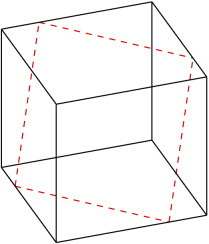
\includegraphics[width=1.6in,angle=-90]{fig1a}}
\put( -90,  0){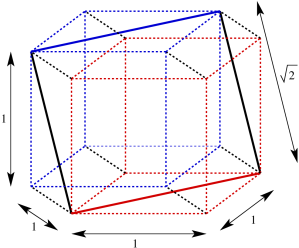
\includegraphics[width=2.3in,angle=  0]{fig1b}}
\put( 100,  5){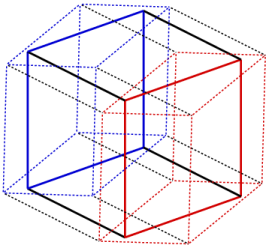
\includegraphics[width=2.0in,angle=  0]{fig1c}}
\end{picture}
\caption{\label{fig:fig1}
(a) Nieuwland's optimal solution to Rupert's original problem where the
    square's vertices divide the cube's edges in the length ratio of 1:3.
(b) The maximal square within a tesseract.
(c) The maximal cube within a tesseract.
}
\label{fig1}
\end{figure*}

\begin{figure*}
\begin{picture}(0,140)
\put(-225,140){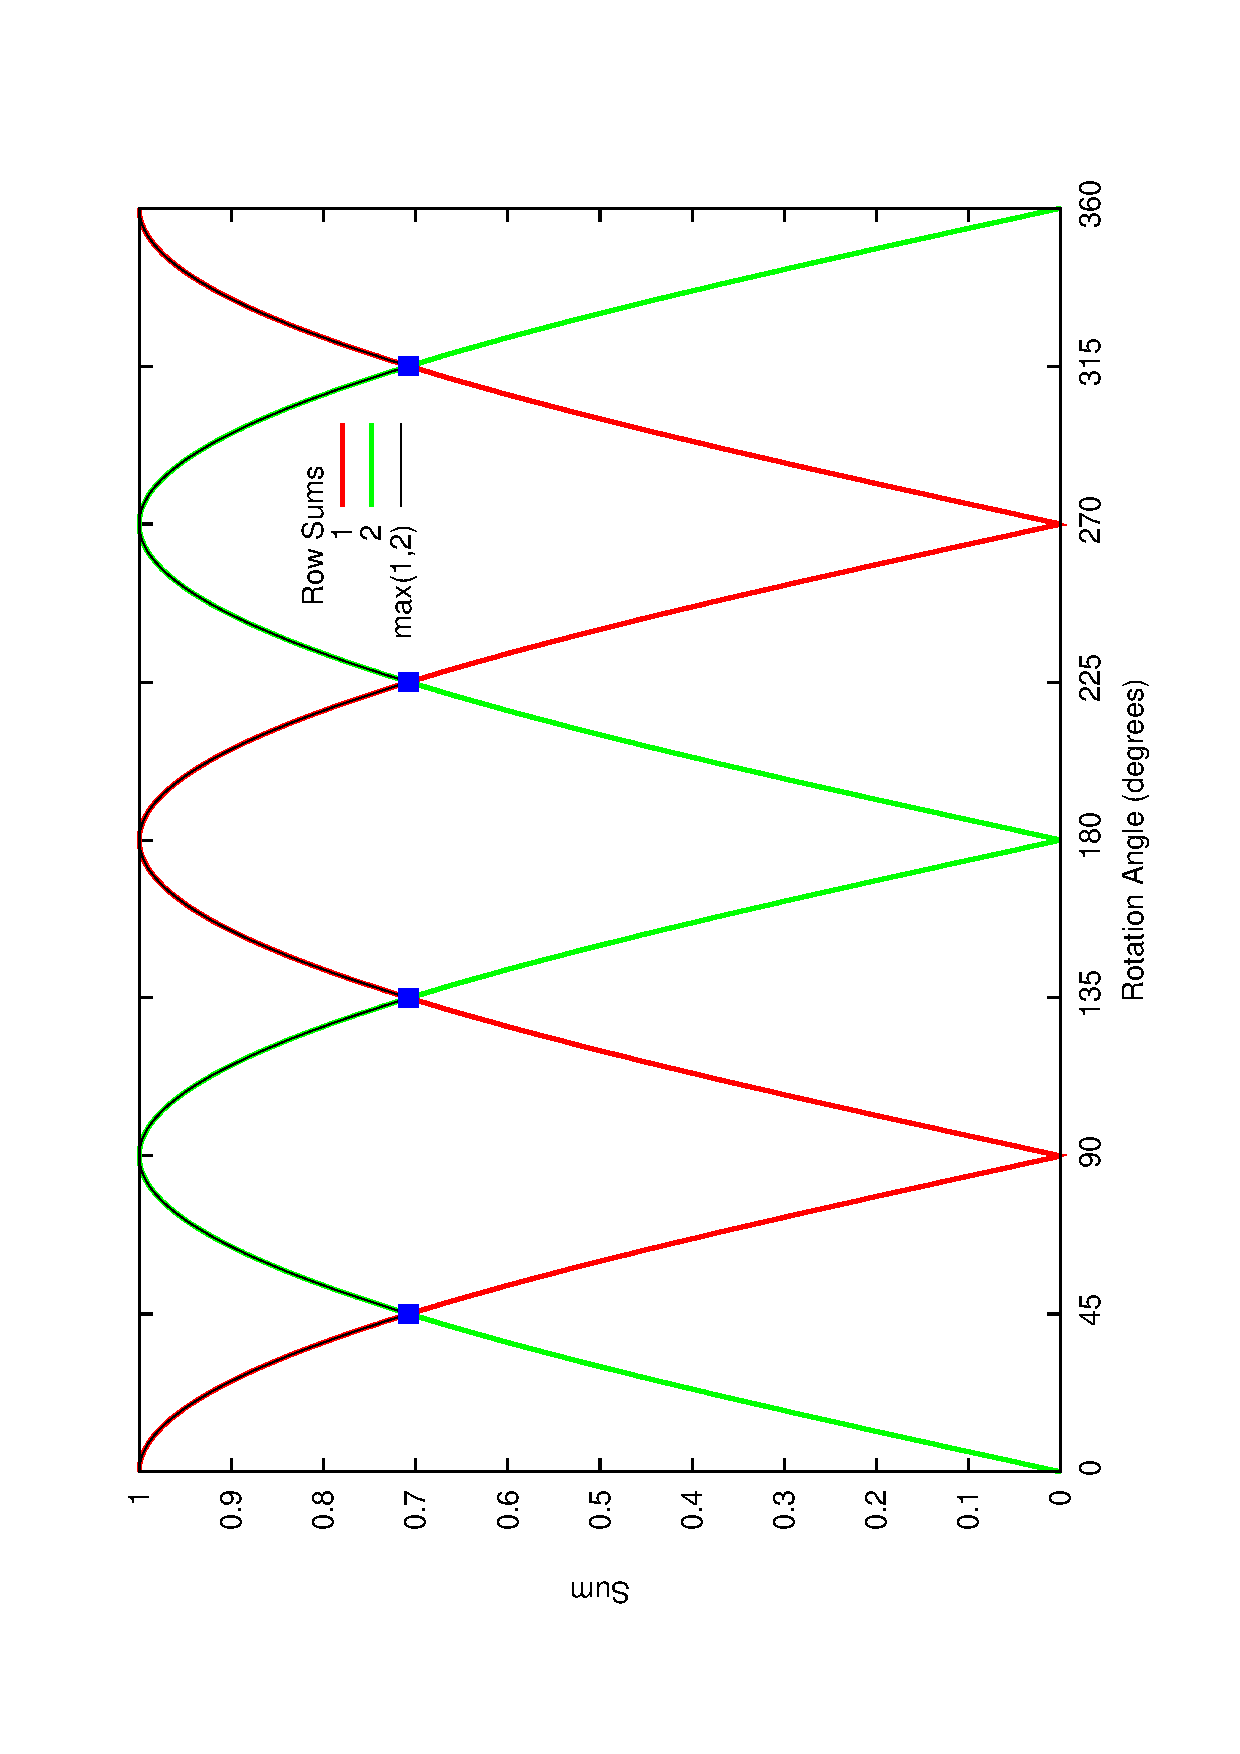
\includegraphics[width=2.0in,angle=-90]{fig2a}}
\end{picture}
\caption{\label{fig:fig2}
(a) Row-sums as a function of angle space for (1,2) problem.
(b) Row-sums as a function of angle space for (2,3) problem.
}
\label{rowsums}
\end{figure*} 


This gave rise to 3 vectors that should form an orthogonal
set and all should have the same length (the 3-cube side length):
\begin{align*}
     s1 & = v1 - v = (   0, x+y, x+y, 0) \\
     s2 & = v2 - v = (-z+1, x-w, y-1, 2) \\
     s3 & = v3 - v = ( z+1, x-1, y-w, 0)
\end{align*}
\begin{align*}
     1)~  0 & = s1 \cdot s2 = ( x+y)(x-w)+(x+y)(y-1)            \\
     2)~  0 & = s1 \cdot s3 = ( x+y)(x-1)+(x+y)(y-w)            \\
     3)~  0 & = s2 \cdot s3 = (-z+1)(z+1)+(x-w)(x-1)+(y-1)(y-w) \\
     4)~l^2 & = s1 \cdot s1 = 2(x+y)^2                          \\
     5)~l^2 & = s2 \cdot s2 = (-z+1)^2+(x-w)^2+(y-1)^2+4        \\
     6)~l^2 & = s3 \cdot s3 = ( z+1)^2+(x-1)^2+(y-w)^2
\end{align*}
Equation (1) and (2) are the same so this gave rise to 5 (non-linear)
equations in 5 unknowns $(x,y,z,w,l)$.  I played with these some and made
some progress but I also gave them to Maple to solve and got $z$ as the
minimum positive (real) solution to:
\begin{align*}
          2z^4 & + 8z^3 + 9z^2 + 10z - 25 = 0 \\
          z & \approx 0.929720699
\end{align*}
\begin{align*}
     x & = \frac{1}{50}(-6z^3 -  4z^2 + 3z + 35)        \\
     y & = \frac{1}{50}( 8z^3 + 22z^2 - 4z + 20)        \\
     w & = \frac{1}{50}( 2z^3 + 18z^2 -  z +  5)        \\
     l & = (x+y)\sqrt{2}                                \\
       & = \frac{1}{50}( 2z^3 + 18z^2 -  z + 55)\sqrt{2}
\end{align*}
These equations gave answers consistent with my numerical results and
what you've told me you've computed.  

\vspace{.15in}

\noindent{\bf Bootstrapping.}
Going from an optimal (m,n) solution to a higher dimensional solution by
using local minimum finding techniques.


Next, I decided to look at the 3 in 7-cube (which also had 4 positional
unknowns and the side length):
\begin{align*}
     v  & = (-1, -x, -y, -1, -1, -1, -1) \\
     v1 & = (-1, -y, -x, -1,  1, -1,  1) \\
     v2 & = (-z, -w, -1,  1, -1,  1, -1) \\
     v3 & = ( z, -1,  w, -1, -1, -1, -1)
\end{align*}
This looks structurally very similar and gave a similar looking set of
equations but the solution (via Maple) is a bit more complicated, $z$ is
the minimum real solution to:
\begin{align*}
          z^8 & - 12z^6 + 4z^5 - 6z^4 + 120z^3 - 208z^2 + 300z - 151 = 0 \\
          z & \approx 0.7227902063
\end{align*}
\begin{align*}
     x & = \frac{1}{456328} (625456 - 484389z +  96148z^2 ...) \\
     y & = \frac{1}{456328} (589343 - 413126z + 286081z^2 ...) \\
     w & = \frac{1}{456328} (492441 -  71263z - 189933z^2 ...) \\
     l & = \sqrt{2(x+y)^2 + 8}
\end{align*}
The expressions for $x$, $y$, and $w$ continue to $z^7$ terms with the
coefficients (mostly) decreasing in magnitude.  Since $0 < z < 1$, this
sort of looks like some type of truncated (convergent?) power series.
The numerical results for these expressions give results consistent with
the numerics.

Then I decided to look at some of the easy examples (one positional
unknown and the side length).  First, I looked at the 3 in 10-cube:
\begin{align*}
     v  & = (-1, -x, -x, -1, -1, -1, -1, -1, -1, -1) \\
     v1 & = (-1, -1, -x, -x,  1, -1,  1, -1,  1, -1) \\
     v2 & = (-x, -x, -1,  1, -1,  1, -1,  1, -1,  1) \\
     v3 & = ( x,  1,  1,  x, -1, -1, -1, -1, -1, -1)
\end{align*}
In this case, all the orthogonal equations are trivially true and two
the length equations are identical.  This is what's left:
\begin{align*}
     l^2 & = 2(x-1)^2 + 12 \\
     l^2 & = 4(x+1)^2
\end{align*}
\begin{align*}
     x & = -3 + \sqrt{14}            \\
     l & = 2(x+1) = l(0) (see below)
\end{align*}
After this a 3 in (3n+10)-cube results have the same form by appending n
copies of (-1,-1,-1) to $v$, (-1,-1,1) to $v1$, (-1,1,-1) to $v2$, and
(1,-1,-1) to $v3$.  The length is given by:  $l(n)^2 = l(0)^2 + 4n$.

To try to complete the 3 in q-cube case, I decided to look at the 3 in
(3n+5)-cube.  For $n=0$ (5-cube), this gave rise to:
\begin{align*}
     l^2 & = 2(x+1)^2     \\
     l^2 & = 4(x-1)^2 + 4
\end{align*}
\begin{align*}
     x & = 3 - \sqrt{6}         \\
     l & = \sqrt{2}(x+1) = l(0)
\end{align*}
and, in general, $l(n)^2 = l(0)^2 + 4n$.

Finally, this made me notice that there seemed to be pattern in the m in
(2m-1)-cube cases.  Namely, there always seemed to be only one
coordinate unknown, the coordinates/vectors had a very simple form, and
they always resulted in two equations in the two unknowns (with
orthogonality guaranteed):
\begin{align*}
     s(1)   & = ( x+1, x+1,    0,   0,    0, ...,    0,   0, 0) \\
     s(2)   & = (   0,   0,  x+1, x+1,    0, ...,    0,   0, 0) \\
            & ...                                               \\
     s(m)   & = (   0,   0,    0,   0,    0, ...,  x+1, x+1, 0) \\
     s(m+1) & = (-x+1, x-1, -x+1, x-1, -x+1,                    \\
            & ~~~~~~~~~~~~~~~~~~~~~~~~~~~~~~~..., -x+1, x-1, 2)
\end{align*}
\begin{align*}
     l^2 & =     2 (x+1)^2     \\
     l^2 & = (2n-2)(x-1)^2 + 4
\end{align*}
\begin{align*}
     x & = \frac{\sqrt{n}}{\sqrt{n}+\sqrt{2}} \\
     l & = \sqrt{2}(x+1) = l(0)
\end{align*}
And, as in previous cases, this extends to the $m$ in (mn + (2m-1))-cube
case:  $l(n)^2 = l(0)^2 + 2n$ for all $n$ and $m$.

\noindent{bf Simulated annealing}
Simulated annealing is a Monte Carlo approach for minimizing such
multivariate functions. The term simulated annealing derives from the
roughly analogous physical process of heating and then slowly cooling a
substance to obtain a strong crystalline structure. In simulation, a minima
of the cost function corresponds to this ground state of the substance. The
simulated annealing process lowers the temperature by slow stages until the
system ``freezes'' and no further changes occur. At each temperature the
simulation must proceed long enough for the system to reach a steady state
or equilibrium. This is known as thermalization. The time required for
thermalization is the decorrelation time; correlated microstates are
eliminated. The sequence of temperatures and the number of iterations
applied to thermalize the system at each temperature comprise an annealing
schedule.  To apply simulated annealing, the system is initialized with a
particular configuration. A new configuration is constructed by imposing a
random displacement. If the energy of this new state is lower than that of
the previous one, the change is accepted unconditionally and the system is
updated. If the energy is greater, the new configuration is accepted
probabilistically. This is the Metropolis step, the fundamental procedure
of simulated annealing. This procedure allows the system to move
consistently towards lower energy states, yet still ‘jump’ out of local
minima due to the probablistic acceptance of some upward moves. If the
temperature is decreased logarithmically, simulated annealing guarantees an
optimal solution.

The original Metropolis scheme was that an initial state of a thermodynamic
system was chosen at energy E and temperature T, holding T constant the
initial configuration is perturbed and the change in energy dE is computed.
If the change in energy is negative the new configuration is accepted. If
the change in energy is positive it is accepted with a probability given by
the Boltzmann factor $exp ‐(dE/T)$.  This processes is then repeated
sufficient times to give good sampling statistics for the current
temperature, and then the temperature is decremented and the entire process
repeated until a frozen state is achieved at $T=0$.

By analogy the generalization of this Monte Carlo approach to matrix
(geometric? combinatoric?) problems is straight forward The current state
of the thermodynamic system is analogous to the current solution to the
combinatorial problem, the energy equation for the thermodynamic system is
analogous to at the objective function, and ground state is analogous to
the global minimum. The major difficulty (art) in implementation of the
algorithm is that there is no obvious analogy for the temperature T with
respect to a free parameter in the combinatorial problem. Furthermore,
avoidance of entrainment in local minima (quenching) is dependent on the
``annealing schedule'', the choice of initial temperature, how many
iterations are performed at each temperature, and how much the temperature
is decremented at each step as cooling proceeds.

\vspace{.15in}

\noindent{\bf Fractal frustration.} 
What is the quantity that measures the ``frustration'' of a cube?  Which
cases of $(m,n)$ are the most frustrated?  How can frustration be read off
the graph of $1/f^2$ versus $m/n$?

\begin{figure*}
\begin{picture}(0,170)
\put(-280,170){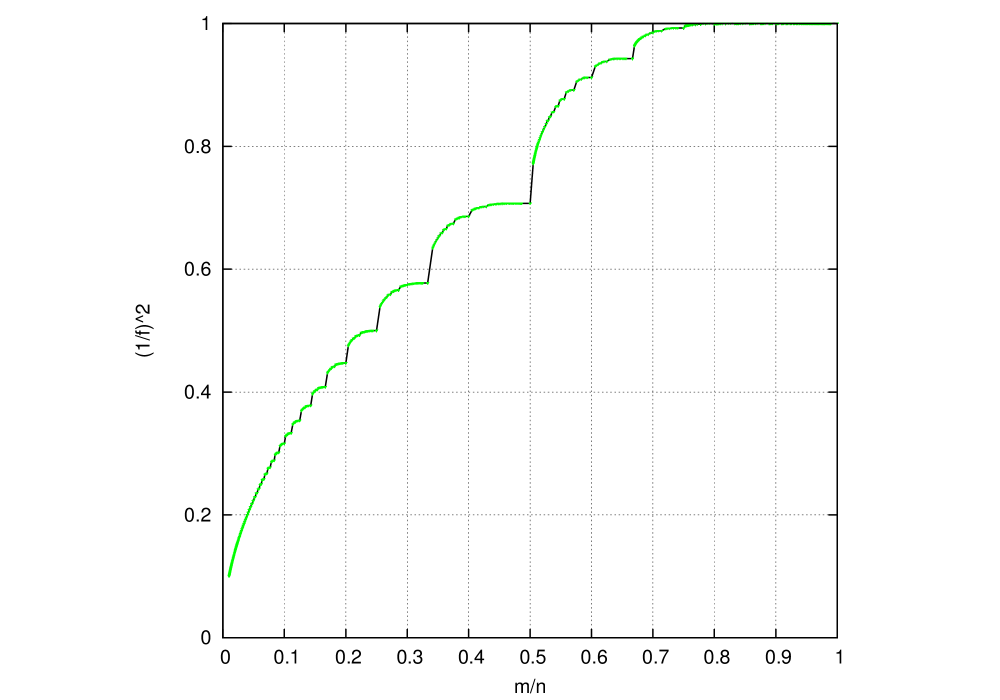
\includegraphics[width=2.5in,angle=-90]{fig3a}}
\put( -20,170){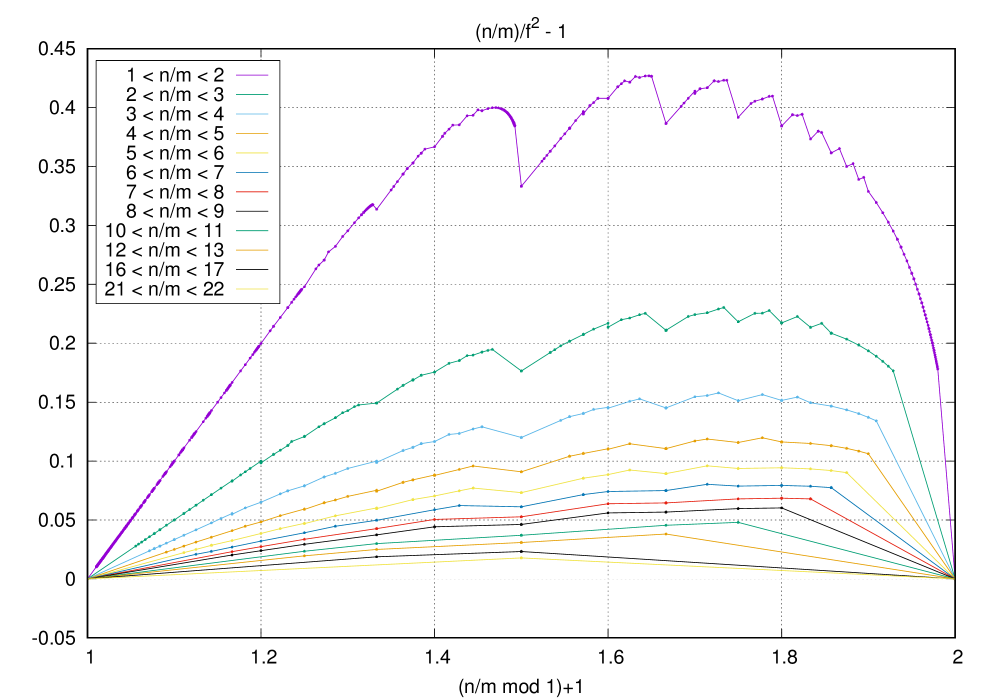
\includegraphics[width=2.5in,angle=-90]{fig3b}}
\end{picture}
\caption{\label{fig:fig3}
(a) Inverse square of the edge length as a function of $m/n$.
(b) $1/f^2 - n/m$ versus $(n/m~\text{mod}~1)+1$.
}
\label{fractalplots}
\end{figure*} 

Figure 3a is $1/l^2$ versus $m/n$, and Figure 3b is $n/l^2-1$ versus $n/m$
graph with all the lobes shifted into an interval of length 1, and some
appropriate closeups.  Discuss our overall impression that there these
graphs/point-sets are self-similar, suggest methods for superimposing them,
and discuss the possible significance.

\noindent{\bf 3-cubes in n-cubes}

The first truly new result that came out of the computer results was a
pattern in the direction cosines for the largest 3‐cube in a 5‐cube.  The
pattern was blah blah blah

This pattern translates in another pattern for the vertices of the 3-cube:
\newcommand{\half}{\frac{1}{2}}
\begin{center}
\renewcommand{\arraystretch}{1.4}
\begin{supertabular}{rrrrr}
    $-\alpha$ & $ \half $ & $-\alpha$ & $-\half $ & $-\half $ \\
    $-\half $ & $ \alpha$ & $-\half $ & $-\alpha$ & $ \half $ \\
    $-\alpha$ & $ \half $ & $ \half $ & $ \alpha$ & $-\half $ \\
    $-\half $ & $ \alpha$ & $ \alpha$ & $ \half $ & $ \half $ \\
    $ \alpha$ & $-\half $ & $ \alpha$ & $ \half $ & $ \half $ \\
    $ \half $ & $-\alpha$ & $ \half $ & $ \alpha$ & $-\half $ \\
    $ \alpha$ & $-\half $ & $-\half $ & $-\alpha$ & $ \half $ \\
    $ \half $ & $-\alpha$ & $-\alpha$ & $-\half $ & $-\half $ \\
\end{supertabular}
\end{center}
where $\alpha = 0.275255128...$
This leads to an edge length = $\sqrt{11 - 4\sqrt{6}} = 1.09637631717731....$

Here is how successive generations of computer experiments approached this
value:
\vspace{-0.05in}
\begin{center}
1.0963763169444 \\
\vspace{-0.02in}
1.0963763170196 \\
\vspace{-0.02in}
1.0963763171015 \\
\vspace{-0.02in}
1.0963763171713 \\
\vspace{-0.02in}
1.0963763171768 \\
\vspace{-0.05in}
....
\end{center}
\vspace{-0.05in}

\vspace{-0.15in}
\begin{figure*}
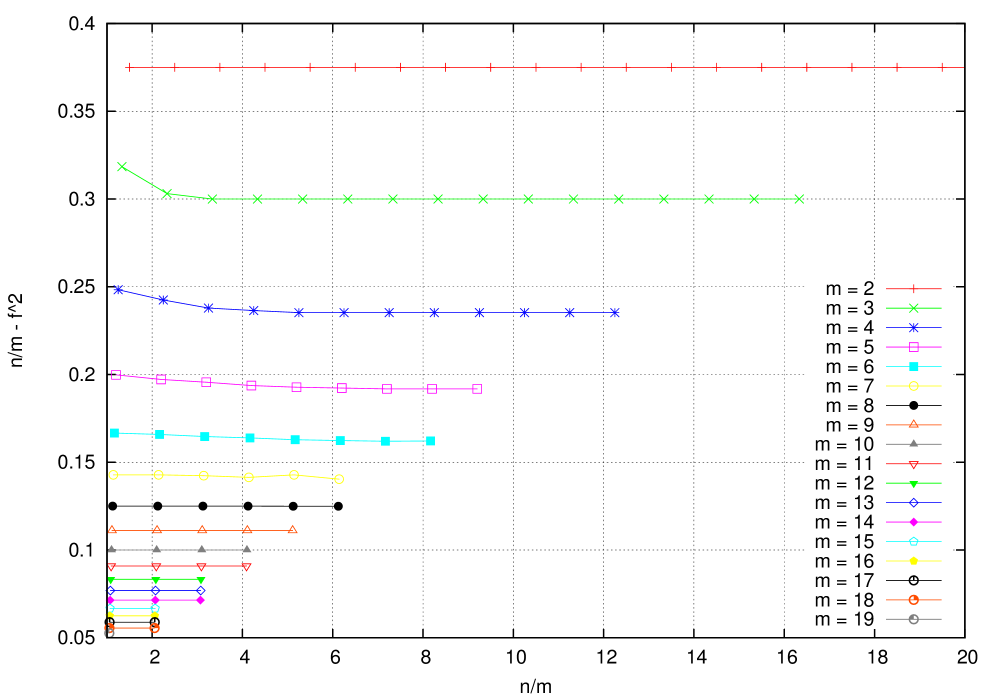
\includegraphics[angle=-90,width=6.5in]{fig4}
\vspace{-0.1in}
\caption{\label{fig:fig4} Energies of families of solutions as a function of $n/m$.}
\label{families}
\end{figure*} 

Extracting families of (m,n) from the previous graphs.  Discuss their
organization, analogies to energy level curves, and their asymptotics.
Introduce the idea of "family extensions" - taking known solutions and
using them to construct lower bound candidates for unknown solutions.
Discuss using them to produce non-constructive lower bounds for unknown
solutions (e.g. using f(m,n) inequalities).  Discuss cases where the
optimal solution candidates obtained by 4(b) seem to correspond to the
"family extensions" after some point in the family (e.g., the (3,5)
family).

In the bound on the $(m-1,m)$ case, the number $2 \cdot 3^{2m-4}$ appears
somewhat naturally.  Is this indicative of an asymptotic exponential form
for the ``correction'' to 1 as m goes to infinity.  An early, crude fit to
the data for small $m$ gave the following:
\begin{equation*}
f(m-1,m)^2 \approx 1 + \frac{67.3}{8.2^m}
\end{equation*}
Notice that this expression is very nearly $1 + 8.2^{2-m}$ which
is eerily reminiscent of the expression from the bound: $1 + \half~9^{2-m}$.

\noindent{\bf Analytic results for $(m-1,m)$ and $(m-2,m)$ (lower bounds)}
We have been able to construct systems of equations for the $(m-1,m)$ family
and the $(m-2,m)$ family.  We have solved these systems iteratively using
Mathematica to arbitrary precision.

\noindent{\bf Other families}
This line of thinking suggests other ``families'' of cases.  For example, a
Fibonacci family:  f(1,2), f(2,3), f(3,5), f(5,8), etc.  These values should
approach a unique answer ‐‐ what is it?  Every irrational can be approached
in a similar way....what are the asymptotics of the approach to these
irrationals?  does it depend on the type of irrational?


\begin{align}
f(m,n) = ...
\label{eq1}
\end{align}
For example, Eq.(\ref{eq1}) refers to the side length of the $m$-cube in the
problem.

\vspace{.15in}

\noindent{\bf Future questions -- taken from our last meeting}


Can we use the Farey tree to organize each of the $m/n$ problems, or to
organize the modular classes?

Does the modular table capture the ’true’ structure of the problem?  Are
there hidden families in the table that need to be exposed?  Do they shed
light on the full problem?

How are the cases $m > n/2$ related to the cases $m < n/2$?  What exactly
is the transformation?  What else can we say about the fractal or self‐
affine properties of the $1/f^2$ plot?

Are there analogs of energies or eigenvalues or ... in this problem? Are
there other quantities besides $1/f$ associated with the global solution?

Using the systems of equations for $(m-1,m)$ and $(m-2,m)$ can the asymtotics
be shown?  Can any of this be proven to be a maximizer instead of simply a
lower bound?

%\section{Acknowledgements}


{\bf Acknowledgments.}
This work was supported by NSF grant number ... 
We have appreciated discussions over the years with K. R. P. DeVicci Shultz, Paul Erd\"os and Raphael Robinson.

\bibliographystyle{apsrev}
\begin{thebibliography} {99}


\bibitem{gardner-colossal} The Colossal Book of Mathematics

\bibitem{glotz1}
\bibitem{glotz2}
\bibitem{steinhardt}
\bibitem{machta}
\bibitem{radin}
\bibitem{wetzel1}
\bibitem{wetzel2}
\bibitem{wallis}
\bibitem{guy} R.K. Guy \textit{Unsolved Problems in Geometry} Springer

\bibitem{phyllo} Phyllotaxis references, Lev Levitov, Y. Couder

\bibitem{chaitin} m-n-m's, packing ellipsoids, P. Chaikin paper
\bibitem{glotzer}
\bibitem{finch}  book, papers
\bibitem{ligocki} thesis?

\bibitem{torquato} a number of papers
\bibitem{conway-torquato} PNAS
\bibitem{ohern} frustration, jamming references
\bibitem{jamming} jamming phase diagram
\bibitem{lubensky} dimension counting, field theory  T.Lubensky
\bibitem{wetzel} j. wetzel papers

%%\bibitem{SZ1989} S. Svetina and B. \v{Z}ek\v{s}, \textit{Eur. Biophys. J.} \textbf{17}, 101 (1989).
%%\bibitem{CG02} R. Capovilla and J. Guven, \textit{J. Phys. A: Math. and Gen.} \textbf{35}, 6233 (2002).

\end{thebibliography}

\end{document}


%\section{Outline} % Old outline for longer paper
%\begin{enumerate}
%
%\item Introduction and history of the problem
%  \vspace{-0.2in}
%  \begin{enumerate}
%  \item set the stage
%  \vspace{-0.1in}
%  \item mention importance of commensurability versus incommensurability
%  \vspace{-0.1in}
%  \item mention matrix formulation
%  \end{enumerate}
%
%\vspace{-0.2in}
%\item History
%
%\vspace{-0.15in}
%\item Modern formulation of the problem
%  \vspace{-0.2in}
%  \begin{enumerate}
%  \item set-up of concentric cubes
%  \vspace{-0.1in}
%  \item n-cube fixed, m-cube variable (or vice versa), $[-1,1]^n$ domain
%  \vspace{-0.1in}
%  \item SO(n) formulation, rotation matrices
 %\end{enumerate}
%
%\vspace{-0.2in}
%\item Basic results and early guesses and conjectures
%  \vspace{-0.2in}
%  \begin{enumerate}
%  \item inequalities on $f(m,n)$
%  \vspace{-0.1in}
%  \item $f > 1$
%  \vspace{-0.1in}
%  \item fundamental conjecture, first (early) version of 'fractal plot'
%  \end{enumerate}
%  
%\vspace{-0.2in}
%\item Numerical methods
%  \vspace{-0.2in}
%  \begin{enumerate}
%  \item simulated annealing
%    \vspace{-0.15in}
%    \begin{enumerate}
%  	\item description of method as applied to geometry
%    \end{enumerate}
%  \vspace{-0.2in}
%	\item annealing schedules
%  \vspace{-0.1in}
%	\item convergence in theory and in practice
%  \vspace{-0.1in}
%  \item visualization of solution space: 'islands' (accessible zones), etc.
%  \end{enumerate}
%
%\vspace{-0.2in}
%\item Numerical discoveries
%  \vspace{-0.2in}
%  \begin{enumerate}
%  \item tables and graphs, full version of fractal plot
%  \vspace{-0.1in}
%  \item numerical evidence for the fundamental conjecture
%  \vspace{-0.1in}
%  \item patterns in the numerics, matrices (Hessenberg)?
%  \vspace{-0.1in}
%  \item the $(m-1,m)$ and $(m-2,m)$ analytics (lower bounds)
%  \vspace{-0.1in}
%  \item $(n-1,n)$ and its asymptotics, other families of problems (Fibonacci?)
%  \end{enumerate}
%  
%\vspace{-0.2in}
%\item Conjectures and future directions (conclusion)
%
%\end{enumerate}
% 
% List of figures:
%\begin{enumerate}
%\item portrait of Prince Rupert
%\vspace{-0.2in}
%\item drawing or photograph of cube sliding through cube
%\vspace{-0.2in}
%\item drawing or photograph of largest square in a cube
%\vspace{-0.2in}
%\item modular table of the (m,n) problems
%\vspace{-0.2in}
%\item plots of $1/f^2$ and $1/f^2 - m/n$
%\vspace{-0.2in}
%\item picture of geometric duality of original problem and matrix formulation
%\vspace{-0.2in}
%\item plots of some families
%\end{enumerate}
% 
